\clearpage
\vspace*{\stretch{2}}%{\fill}
\begin{center}
\begin{minipage}{.75\textwidth}
\section{Análisis previo y funcional}

Una vez revisada la idea general que se busca en este TFG y las tecnologías de las que hacemos uso para lograrlo, en este capítulo mostramos el análisis previo (requisitos) y el funcional (visión de alto nivel de los distintos módulos funcionales principales de que consta el sistema). % \pagebreak
\end{minipage}
\end{center}
\vspace{\stretch{3}} % \vfill % equivalent to \vspace{\fill}
\clearpage% https://tex.stackexchange.com/questions/70714/center-horizontally-and-vertically-a-block-of-text

\subsection{Objetivo y análisis de requisitos}
El objetivo de nuestro sistema de sensado móvil colaborativo, asimétrico con beneficio para todos los participantes, es implantar un sistema capaz de ofrecer un servicio de conexión WiFi a Internet a cambio de datos procedentes del sensor de audio (micrófono) del dispositivo móvil que utilice el cliente (aunque no limitado a este tipo de dispositivos). Para ello utilizamos una combinación de hardware y aplicaciones software ya existente, programando desde cero los módulos restantes.

Los requisitos del sistema son los siguientes:

\begin{itemize}
\item Soporte para múltiples navegadores y sistemas operativos, incluyendo móviles.
\item Mínima interacción con el usuario: sólo se requiere de la provisión de permisos la primera vez que se utiliza el sistema en un Punto de acceso determinado. Si se cambia de punto de acceso es necesario volver a dar permisos.
\item Que proporcione más datos aparte de los del sensor de audio.
\item Proveer distintos modos de conexión a Internet.
\end{itemize}

El primer requisito podría alcanzarse de forma sencilla. Dado que a priori vamos a emplear tecnología Web basándonos en estándares que todos los navegadores modernos deben estar preparados para procesar no se requeriría instalar ninguna aplicación o complemento de navegador adicional en los clientes del servicio. Además, se tendría en cuenta el diseño Web responsivo, de forma que la visualización del contenido se adapte al tamaño y características del dispositivo. Sin embargo, existen ciertas particularidades.

Los estándares utilizados para implantar la funcionalidad de captura de sonido, como WebRTC y MediaStream Recording, están aún abiertos y tienen poco tiempo, por lo que solo están soportados en versiones muy recientes de los navegadores o incluso, hasta hace poco tiempo, únicamente en sus versiones experimentales. Por ejemplo, Safari, el navegador Web de Apple por defecto para sus ordenadores con MacOS y los dispositivos iOS, ha comenzado a trabajar con los estándares WebRTC y relacionados hace tan solo un año, anunciando su compatibilidad para la versión 11 del navegador que salida en Septiembre de 2017. Por el momento, para Safari solo puede encontrarse una compatibilidad preliminar en su versión para desarrolladores, Safari Technology Preview \cite{SafariWebRTC}.

En cuanto al segundo requisito, se plantea que las únicas interacciones que tenga que hacer el usuario con el servicio intermedio de portal cautivo antes de obtener acceso a Internet sea la concesión de permisos de ubicación y captura de audio y otro botón para comenzar el proceso de conexión, representando una ventaja sobre otros sistemas de portal cautivo donde hay múltiples redirecciones, procesos de creación de cuentas de usuario y de inicio de sesión.

Para alcanzar el tercer requisito se trata de aumentar la usabilidad del servicio más allá de capturar un fragmento de sonido, obteniendo también su ubicación y una marca de tiempo para poder hacer análisis estadísticos, mapeos de niveles de señal 3D en función del tiempo, etc.

El cuarto requisito ha surgido a partir de las pruebas realizadas y el desarrollo iterativo e incremental del sistema. Esto es, inicialmente se especificó únicamente un modo de conexión a Internet debiendo el cliente Web mantener abierta la pestaña del navegador Web en la que se proporcionó el permiso para acceder al micrófono. La aplicación javascript de esa pestaña capturaba un fragmento de audio de 5 segundos cada 3 minutos. La ventaja es que la ofrece al usuario una conexión más estable. La desventaja es que retiene el control del micrófono en modo exclusivo para esa aplicación Javascript. Haciendo desarrollos incrementales se detectó este comportamiento a priori no explícito, por lo que se observó que este comportamiento no sería adecuado para aquellos usuarios que quisieran hacer uso del micrófono a la vez que está conectado a Internet (por ejemplo, mensajería de audio vía aplicaciones de mensajería instantánea). Por ello, en segundo lugar se especificó como requisito previo que pudiera existir un nuevo modo de conexión a Internet. Esto es, ofrecer un tiempo de conexión fijo de 30 minutos a cambio de un único archivo de audio inicial, tras lo cual podría cerrarse la pestaña del navegador de la Aplicación Web y hacer uso libre del micrófono del dispositivo durante este tiempo.

\subsection{Análisis previo}

El sistema está compuesto de varios elementos que interactúan entre sí. A continuación se ofrece un resumen del funcionamiento de cada elemento, los módulos que lo componen y las tareas asociadas a los mismos:

\begin{itemize}
\item \emph{Hardware necesario}: se supone que en el local a monitorizar ya existe un acceso a Internet al cual se puede conectar un Punto de acceso WiFi. Por ello, únicamente es necesario una Raspberry Pi 3 Model B con el sistema operativo Raspbian, un módulo software controlador del módulo WiFi 802.11 (Hostapd) para habilitar su funcionamiento como Punto de Acceso, el software de control de acceso y el servicio de portal cautivo. La configuración de este software para que funcionara adecuadamente llevó mucho tiempo debido a la falta de información o bien información obsoleta sobre estas aplicaciones. Por ello hubo de realizarse muchas pruebas de ensayo-error hasta que definitivamente pudimos dar con la configuración correcta.
\item \emph{Aplicaciones software configurables}: para proveer el acceso a Internet es necesario utilizar las siguientes aplicaciones que ya existen y que se deben configurar adecuadamente. Destacar que esta tarea de configuración no es sencilla, debido a la falta de información veraz, la obsolescencia de la información existente y la dificultad de instalarlos en la Raspberry Pi 3. Por este motivo hubo de realizar múltiples pruebas de ensayo y error hasta dar con la configuración adecuada, cuyas ideas generales proporcionamos a continuación:
\begin{itemize}
\item \emph{Control de acceso}:
\begin{itemize}
\item \emph{RADIUS}: necesario para la autenticación de los usuarios. Se utilizó el daloRADIUS, para la gestión interna del acceso de usuarios, recibiendo las credenciales proporcionadas por el servicio de portal cautivo y gestionando su conexión.
\item \emph{CovaChilli y su entorno}: necesario para redirigir correctamente los paquetes entrantes (autorizados previamente por RADIUS) desde la interfaz inalámbrica a la interfaz cableada y viceversa. Aquí hubo que configurar las ubicaciones de nuestro portal cautivo propio, los ajustes de autenticación de usuarios y habilitar el uso de \acrshort{SSL}.
\end{itemize}
\item \emph{Node.js}: necesario para implementar el servidor donde alojar nuestro portal cautivo, recibir y procesar los ficheros de audio generados e instalar servicios de monitorización del mismo.
\end{itemize}
\item \emph{Aplicaciones software desarrolladas desde cero}:
\begin{itemize}
\item \emph{Portal cautivo}: enlaza a los usuarios con el control de acceso mediante un sistema de control de usuarios intermedio, realizando también la tarea de captura y almacenamiento de archivos de audio procedentes de los micrófonos de los dispositivos, que es lo que da sentido al sistema global. Su funcionalidad se detalla a continuación. Su funcionalidad básica es:
\begin{itemize}
\item \emph{Servidor Web}: implantado con Node.js, se encargaría de lo siguiente:
\begin{itemize}
\item Servir la aplicación Web a los usuarios que se conecten a la red.
\item Recibir y almacenar archivos de audio de los usuarios conectados.
\item Llevar un control de los usuarios a los que se ha dado acceso a Internet.
\item Informar a los clientes del estado del servidor.
\end{itemize}
\item \emph{Cliente Web}: implantado con , HTML, CSS y JavaScript, y se encarga de lo siguiente:
\begin{itemize}
\item Ser el punto de entrada de los usuarios al sistema, ofreciendo dos modalidades de conexión diferentes.
\item Comprobar el estado del servidor.
\item Adquirir datos de ubicación y marca de tiempo de los usuarios.
\item Capturar una señal de audio de los usuarios en intervalos constantes.
\item Enviar la señal de audio al servidor.
\item Pedir credenciales de usuario al servidor.
\item Conectar al usuario a Internet con las credenciales recibidas. 
\end{itemize}
\end{itemize}
\end{itemize}
\end{itemize}

\subsection{Análisis funcional}

La estructura global del sistema podría entenderse como un conjunto de módulos que proporcionen un nivel de abstracción adicional, útil para comprender el sistema. Después, pueden dividirse estos módulos en otros submódulos que representen las funciones desempeñadas por cada uno de ellos individualmente en el sistema global. Muchos de estos submódulos representan instalaciones de \emph{software} completas en sí mismas.

Considerando esta aproximación al sistema podemos representar el mismo como una combinación de tres módulos o capas, todos ellos implantados sobre el \emph{hardware} anteriormente mencionado y interrelacionados entre sí. En la Figura \ref{modulos} se muestra el conjunto de módulos principales considerados.

\begin{figure}[!t]
\begin{center}
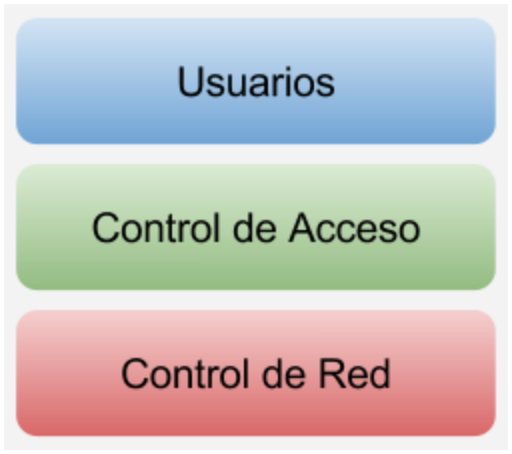
\includegraphics[width=0.75\linewidth]{./4_AnalisisFuncional/Img/modulos.png}
\end{center}
\caption{Diagrama de módulos funcionales}
%\source{http://coova.github.io/CoovaChilli/}
\label{modulos}
\end{figure}

Un primer módulo de \emph{Usuarios} consiste tanto en la única interfaz que los usuarios del sistema (\emph{Vista}) como el servidor que proporciona dicha interfaz junto a un primer control de usuarios (\emph{Controlador} y una parte del \emph{Modelo} relacionado con las acciones que lleva a cabo el servidor). El segundo módulo es el de \emph{Control de Acceso}, que incluye todo el software dedicado a esta gestión, formado por CoovaChilli y su entorno (\emph{Observador}). Por último se halla el módulo de Control de Red, que incluye todo el \emph{software} que permite a la Raspberry Pi funcionar como Punto de Acceso inalámbrico y la configuración de las diferentes redes que entran en juego en el sistema.

Huelga decir que, si bien los clientes del servicio solo interactuarían con el módulo de Usuarios, los otros dos módulos del sistema son accesibles a un administrador, que se encargaría de su correcta configuración inicial y posterior mantenimiento.

\subsubsection{Módulo Usuarios}
Es el módulo de más alto nivel y el único punto de contacto visible de los usuarios con el servicio. Está compuesto de cinco submódulos; un grupo de tres submódulos que interactúan entre sí para proporcionar el servicio, que son la aplicación Web, el servidor y el control de usuarios; un módulo que hace de interfaz con el módulo inferior de Control de Acceso, biblioteca CoovaChilli; y un último módulo que configura y controla el uso de esta interfaz. En la Figura \ref{moduloUsers} se muestra un esquema básico de las relaciones entre los diferentes submódulos que conforman la capa de Usuarios.

\begin{figure}[!t]
\begin{center}
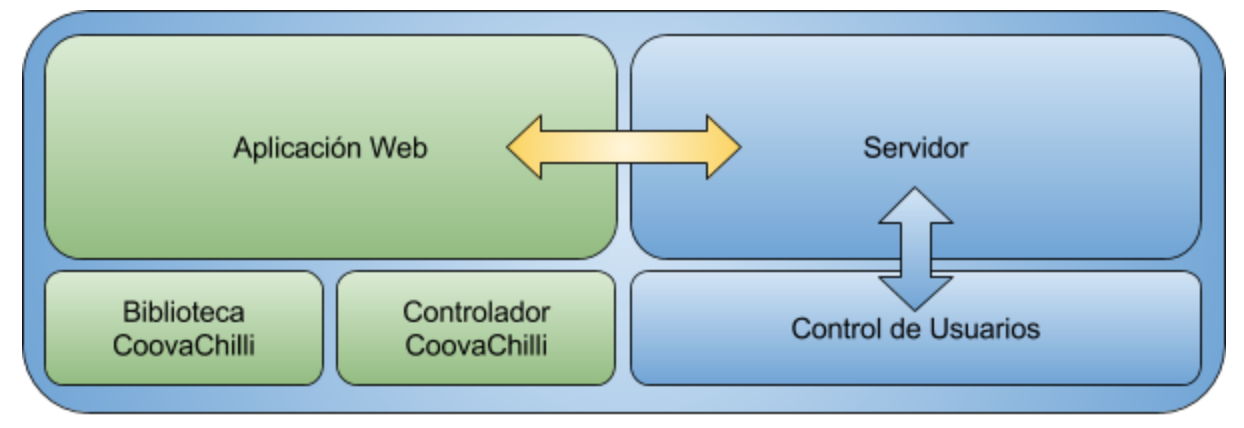
\includegraphics[width=0.75\linewidth]{./4_AnalisisFuncional/Img/moduloUsers.png}
\end{center}
\caption{Diagrama de submódulos del módulo Usuarios}
%\source{http://coova.github.io/CoovaChilli/}
\label{moduloUsers}
\end{figure}

La \emph{Aplicación Web} contiene los datos del portal cautivo al que se redirigen los clientes cuando traten de conectarse a la red inalámbrica. Sus funciones, ya adelantadas en el análisis previo pero ampliadas aquí, son:

\begin{itemize}
\item Adquirir los permisos de ubicación y captura de audio del usuario.
\item Comprobar el estado del servidor para evitar hacer el proceso si este está lleno (haciendo imposible la conexión al servicio).
\item Capturar una muestra corta de dicho audio una única vez o a intervalos regulares, dependiendo del modo de conexión escogido, y enviarla al servidor.
\item Recibir las credenciales de usuario enviadas por el servidor, utilizando como nombre de archivo las coordenadas y la marca de tiempo de la última consulta de geolocalización.
\item Gestionar la conexión de los usuarios con las credenciales recibidas, todo ello por medio de la configuración y las funciones de la biblioteca CoovaChilli y su controlador.
\item Además, está programada para cerrar la conexión si su pestaña del navegador se cierra o se recarga de alguna forma.
\end{itemize}

En la Figura \ref{flujoSistema} se muestra un diagrama de flujo con la funcionalidad básica del sistema en una primera conexión. En este diagrama se omite la fase de elección de los diferentes modos de conexión.

\begin{figure}[!t]
\begin{center}
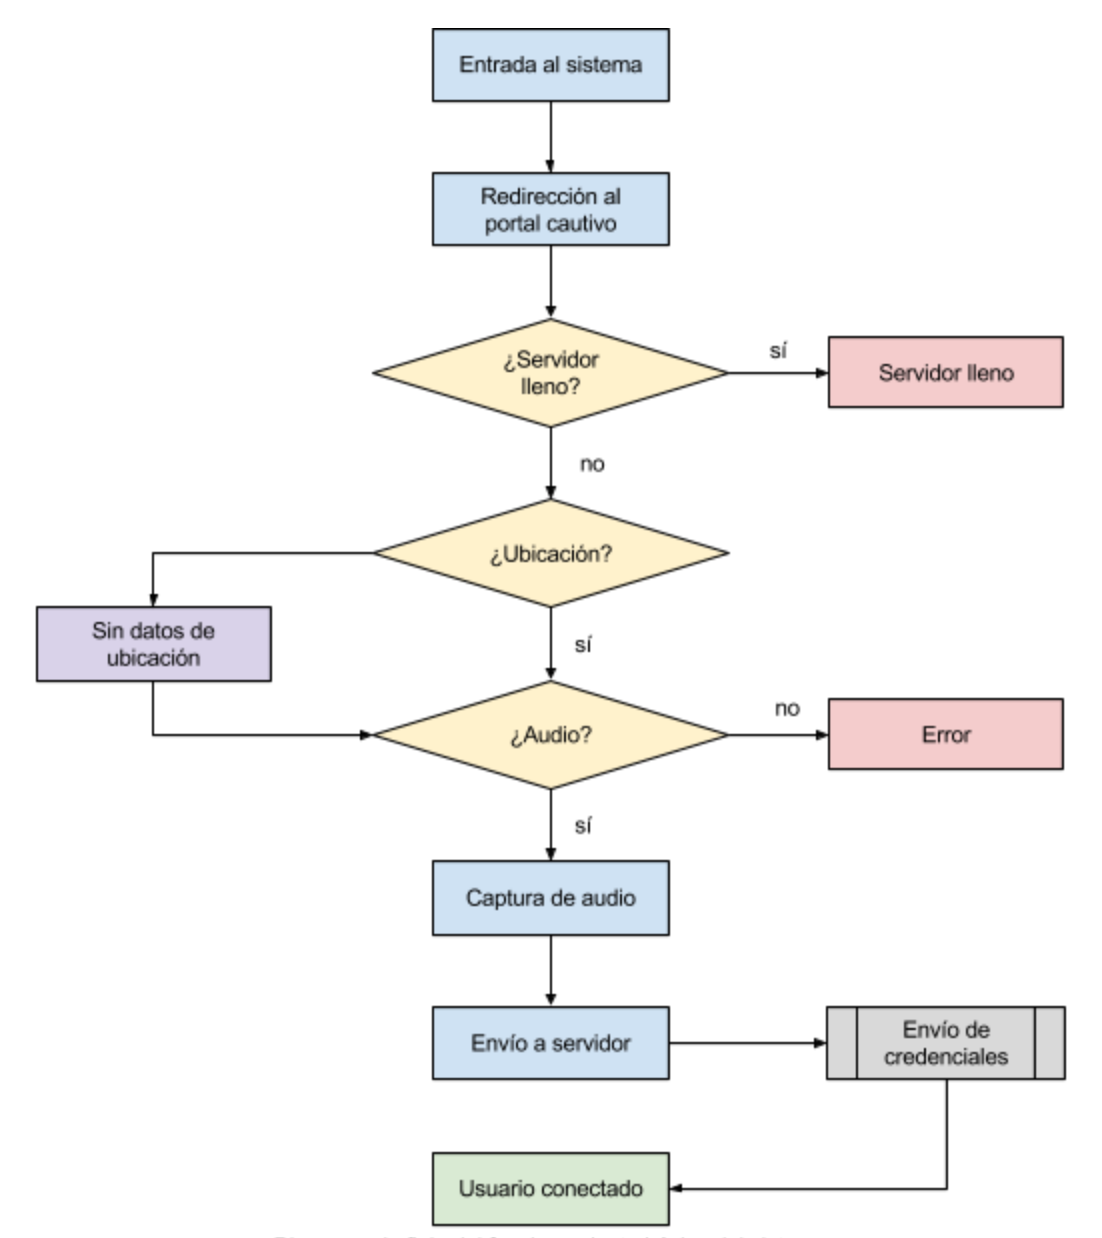
\includegraphics[width=0.75\linewidth]{./4_AnalisisFuncional/Img/flujoSistema.png}
\end{center}
\caption{Diagrama de la funcionalidad de la conexión a Internet a través del portal cautivo modificado}
%\source{http://coova.github.io/CoovaChilli/}
\label{flujoSistema}
\end{figure}

Todas las consultas que ocurren entre la aplicación Web y el servidor utilizan peticiones GET y POST gestionadas mediante AJAX.

El \emph{Servidor} se encarga de enviar la Aplicación Web en forma de HTML estático a los usuarios que realicen peticiones al mismo, y de comunicarse con los clientes y el Control de Usuarios para aportar la funcionalidad deseada. Sus funciones ampliadas son:

\begin{itemize}
\item Servir la Aplicación Web.
\item Comprobar el estado del servidor comunicándose con el \emph{Control de Usuarios}, informando a la \emph{Aplicación Web} si el servicio está disponible o por el contrario está lleno, con lo que no podría prestarse el servicio.
\item Si recibe un archivo de audio de un cliente que aún no tiene credenciales asignadas, pide al \emph{Control de Usuarios} unas credenciales que se encuentren disponibles en su base de datos y las almacena a la espera de que la \emph{Aplicación Web} las pida.
\item Enviar las credenciales almacenadas a la \emph{Aplicación Web}, informando al \emph{Control de Usuarios} para que marque dichas credenciales como utilizadas.
\item Recibir notificaciones de desconexión de usuarios por parte de la \emph{Aplicación Web} y pasar dicha información al \emph{Control de Usuarios} para marcar un usuario como libre en la base de datos.
\end{itemize}

Para llevar a cabo todas estas tareas se utiliza Node.js, los módulos de npm \emph{Express} para la funcionalidad de servidor, \emph{Formidable} para la gestión de archivos de audio entrantes. \emph{Body-Parser} para leer determinadas variables procedentes de la Aplicación Web y los módulos del núcleo de Node.js, Fs para acceder al sistema de archivos y escribir en él y Path para trabajar con las rutas de archivos y directorios.

El \emph{Control de Usuarios} se encarga de gestionar los usuarios activos e inactivos por medio de una base de datos sencilla, implementada con dos archivos JSON, uno para cada modo de conexión, y dos archivos JavaScript que controlan a cada archivo JSON por separado actuando como módulos Node.js del \emph{Servidor}. Si la cantidad de usuarios posible se hiciera lo suficientemente grande, este módulo y su archivo JSON podrían ser reemplazados por una aplicación de base de datos más potente (MySQL, MongoDB...). Los archivos base de datos JSON constan de un \emph{array} de usuarios, cada uno de ellos con los siguientes atributos:

\begin{itemize}
\item \emph{id}: un número entero igual o superior a 0 que actúa como identificador interno de usuario.
\item \emph{username}: el nombre del usuario.
\item \emph{password}: la contraseña del usuario.
\item \emph{isActive}: una variable booleana, que tiene la asignación \emph{true} si el usuario está ocupado y \emph{false} en caso contrario.
\end{itemize}

Las funciones de los archivos JavaScript que controlan al archivo JSON anterior son:

\begin{itemize}
\item Buscar un usuario inactivo en el archivo de base de datos, devolviendo el identificador y las credenciales de dicho usuario si lo hubiera.
\item Asignar usuarios como activos o inactivos escribiendo en el atributo \emph{isActive} correspondiente.
\item Hacer externas las credenciales del usuario seleccionado para que el \emph{Servidor} pueda accederlas y hacer sus operaciones.
\end{itemize}

La biblioteca \emph{CoovaChilli} es un archivo JavaScript denominado \verb+ChilliController.js+, proporcionado por la instalación de CoovaChilli en el directorio \verb+/etc/chilli/www/+. Se encarga de enlazar la Aplicación Web con la interfaz JSON de CoovaChilli creando el objeto global \emph{chilliController}, que puede utilizar los métodos descritos en el capítulo anterior para gestionar la conexión y desconexión de usuarios al servicio.

Por último, el \emph{Controlador CoovaChilli} es un archivo JavaScript de configuración, que modifica los atributos por defecto del objeto \emph{chilliController} creado por la biblioteca CoovaChilli y enlaza los métodos de dicho objeto con acciones concretas de la Aplicación Web.

\subsubsection{Módulo Control de Acceso}
Este módulo está basado en instalaciones y configuraciones de \emph{software} concernientes la gestión interna del control de acceso al servicio. Puede dividirse en tres submódulos: \emph{CovaChilli}, \emph{Servidor RADIUS} e \emph{Interfaz Web de control de RADIUS}. Hemos preferido denominar a los dos primeros submódulos con los nombres originales del software utilizado por claridad. La funcionalidad que aprovechamos de estas aplicaciones es la que tienen, en particular, para este TFG. La tarea aquí básicamente es encontrar, tarea no sencilla, la instalación y configuración adecuada de estos submódulos. El tercer submódulo es una implantación propia que llevó mucha dificultad debido a la complejidad de la conexión entre estos submódulos. En la Figura \ref{moduloControlAcceso} se muestra un diagrama de estos submódulos.

\emph{CoovaChilli} es el submódulo que se encarga de la mayor parte del trabajo. Redirige las conexiones entrantes no autenticadas al portal cautivo implantado en el módulo de \emph{Usuarios} y mantiene un contacto constante con el \emph{Servidor RADIUS}. Como parte de este submódulo se destaca también la \emph{Interfaz JSON}, que viene incluida en la instalación de CoovaChilli y hace posible comunicar dicho \emph{software} con nuestra \emph{Aplicación Web}.

El \emph{Servidor RADIUS} es el gestor de AAA requerido por CoovaChilli para funcionar, aunque es posible implantar otro tipo de servicios para llevar a cabo esta gestión, en este TFG se ha utilizado la aplicación \emph{FreeRADIUS}. En este submódulo también se incluye todo aquel \emph{software} que sea obligatorio para que el servidor funcione, como las instalaciones de bases de datos y su respectiva configuración.

Por supuesto, para que el sistema pueda funcionar, la base de usuarios del \emph{servidor RADIUS} y la existente en los archivos JSON del submódulo \emph{Controlador de Usuarios}, pertenecientes al módulo de de \emph{Usuarios}, ha de ser la misma.

Opcionalmente, puede instalarse un administrador gráfico del Servidor RADIUS para hacer más intuitiva su gestión. En este caso se incluye el submódulo \emph{Interfaz Web de control RADIUS}, representada por una instalación del administrador Web daloRADIUS funcionando sobre el servidor Web \emph{NGINX}.

\begin{figure}[!t]
\begin{center}
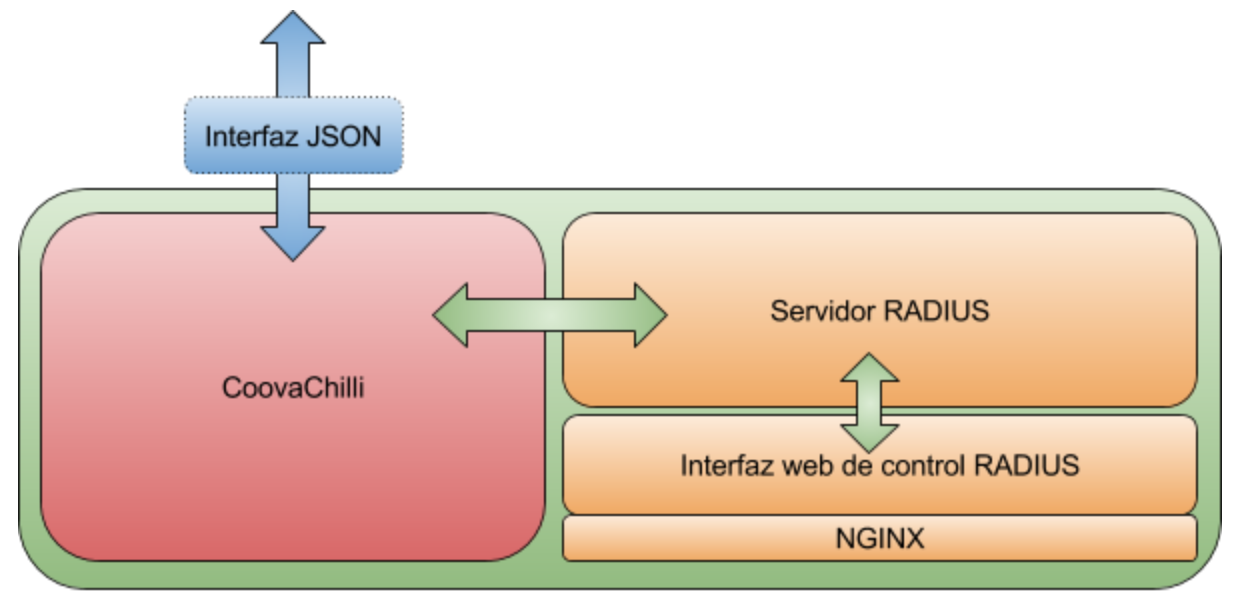
\includegraphics[width=0.75\linewidth]{./4_AnalisisFuncional/Img/moduloControlAcceso.png}
\end{center}
\caption{Diagrama de submódulos del módulo Control de Acceso}
%\source{http://coova.github.io/CoovaChilli/}
\label{moduloControlAcceso}
\end{figure}

\subsubsection{Módulo Control de Red}
El módulo de \emph{Control de Red} es el de más bajo nivel de nuestro sistema, encargado de configurar y gestionar el comportamiento de los componentes \emph{hardware} de la Raspberry Pi. Puede dividirse en tres submódulos: la \emph{Configuración de las Interfaces de Red}, \emph{Hostapd} y el propio dispositivo sobre el que opera todo el servicio: la \emph{Raspberry Pi} con el sistema operativo Raspbian. Hemos preferido denominar a los módulos segundo y tercero como la aplicación original y el hardware por simplicidad para que se entienda que en esos módulos la tarea principal fue la de instalarlos y configurarlos adecuadamente (recurriendo a la técnica de ensayo y error en la mayoría de la veces). En la Figura \ref{moduloControlRed} se muestra el esquema de submódulos de este módulo. 

\begin{figure}[!t]
\begin{center}
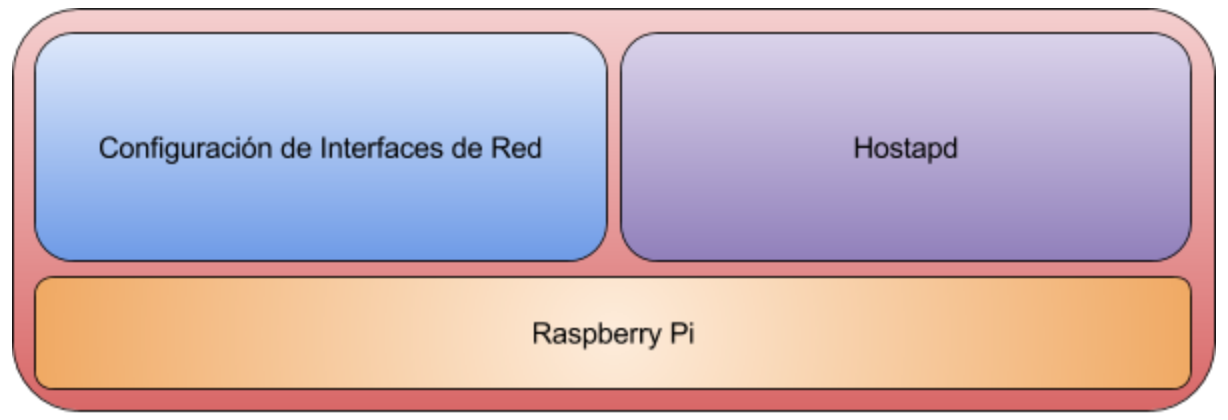
\includegraphics[width=0.75\linewidth]{./4_AnalisisFuncional/Img/moduloControlRed.png}
\end{center}
\caption{Diagrama de submódulos del módulo de Control de Red}
%\source{http://coova.github.io/CoovaChilli/}
\label{moduloControlRed}
\end{figure}

El submódulo \emph{Configuración de Interfaces de Red} consiste en utilizar las herramientas instaladas en Raspbian (adquiriendo las que no estén disponibles por defecto) para implantar y configurar las redes necesarias para el funcionamiento del sistema. Las dos redes principales que intervienen, la cableada Ethernet \emph{eth0} y la inalámbrica \emph{wlan0}, varían su configuración según el entorno en el que se encuentren. La \emph{wlan0} debe configurarse con IP estática y se le debe asignar la red correspondiente, dado que va a ser nuestro Punto de Acceso WiFi.

La configuración de \emph{eth0} depende de la red que proporciona el acceso a Internet al sistema. Por ejemplo, la red cableada de la Universidad (donde hicimos pruebas) solo es accesible cuando la interfaz tiene una IP determinada en el punto de conexión, no pudiendo conectarse si no se asigna la IP adecuada. En una instalación de Internet casera puede configurarse la interfaz sin IP y dejar que el DHCP del router de la instalación asigne una dirección adecuada para establecer su red local.

Esta configuración incluye el paso necesario de habilitar el \emph{flag} del \emph{kernel} Linux del sistema operativo Raspbian para que permita el proceso de reenvío de paquetes IP, o IP forwarding, desde la interfaz cableada a la inalámbrica y viceversa. Sin este paso la instalación de CoovaChilli, que basa su funcionalidad de paso de paquetes entre interfaces mediante el uso de órdenes \emph{iptables} de Linux \cite{TUNTAP2}, no podría funcionar.

\begin{figure}[!ht]
\begin{center}
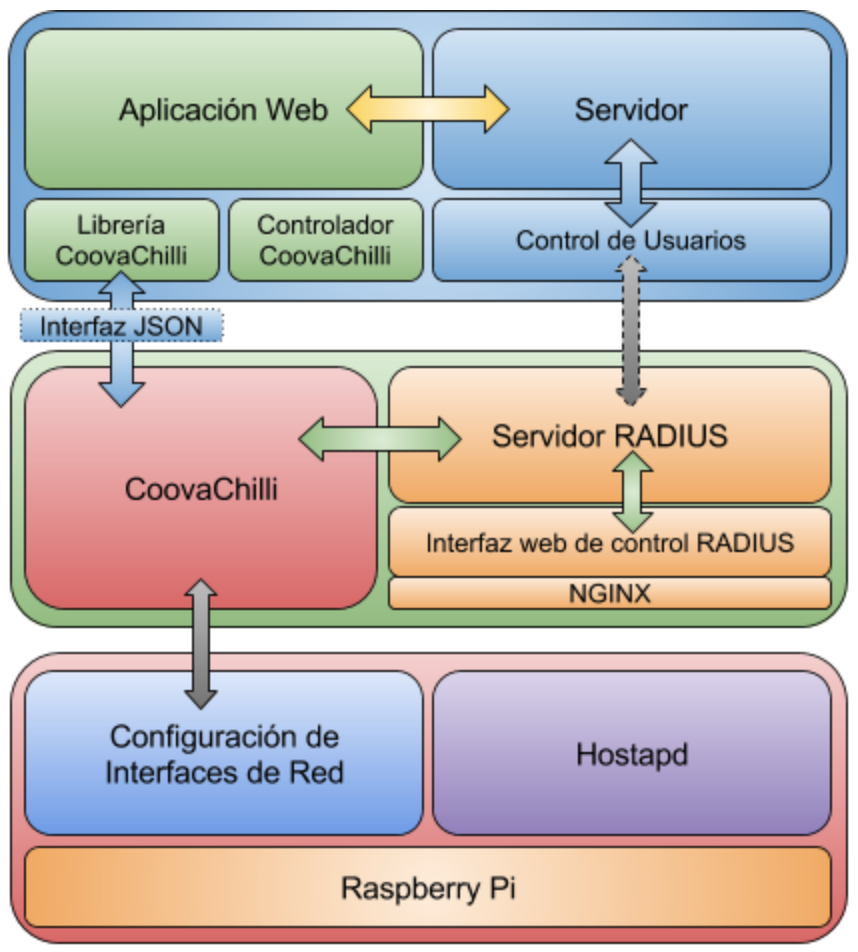
\includegraphics[width=0.75\linewidth]{./4_AnalisisFuncional/Img/modulosTotal.png}
\end{center}
\caption{Esquema completo de los módulos funcionales del sistema}
%\source{http://coova.github.io/CoovaChilli/}
\label{modulosTotal}
\end{figure}

Como también se adelantó en el anterior capítulo, Hostapd es un servicio que se ejecuta en segundo plano, configurando y permitiendo el uso de la interfaz inalámbrica \emph{wlan0} como punto de acceso WiFi 802.11n para que los clientes se conecten a nuestro servicio.

El submódulo \emph{Raspberry Pi}, con el sistema operativo Raspbian, proporciona las interfaces de red necesarias, \emph{software} y dependencias para instalar todo el ecosistema y las opciones de configuración de red que hacen posible la implementación total del servicio.

Para una mayor entendimiento global de todo el sistema instalado, configurado y desarrollado, en la Figura \ref{modulosTotal} se presenta un diagrama que engloba los tres módulos, incluyendo sus submódulos, y las interrelaciones existentes entre los mismos.